\documentclass[11pt,twocolumn]{article}

% --- Codificación y lenguaje ---
\usepackage[T1]{fontenc}
\usepackage[utf8]{inputenc}
\usepackage[spanish]{babel}

% --- Matemática y unidades ---
\usepackage{amsfonts,amssymb,amsmath,amsthm}
\usepackage{siunitx}
\sisetup{
  per-mode=symbol,
  separate-uncertainty=true,
  output-decimal-marker={,}
}

% --- Gráficos y tablas ---
\usepackage{graphicx}
\usepackage{caption}
\usepackage{subcaption}
\usepackage{booktabs}
\usepackage{array}
\usepackage{makecell}
\usepackage{multirow}

% --- Varios útiles ---
\usepackage[margin=2cm]{geometry}
\setlength{\columnsep}{0.7cm}
\raggedbottom
\usepackage{enumitem}
\setlist[itemize]{leftmargin=*, itemsep=2pt, topsep=2pt}
\setlist[enumerate]{leftmargin=*, itemsep=2pt, topsep=2pt}
\usepackage{csquotes}
\usepackage{cuted}
\usepackage{float}
\usepackage{placeins}
\usepackage[dvipsnames]{xcolor}
\usepackage{tikz}
\usetikzlibrary{calc}

% --- Estética de tablas y figuras ---
\captionsetup{font=small,labelfont=bf}
\AtBeginDocument{\renewcommand{\tablename}{Cuadro}}
\renewcommand{\arraystretch}{1.12}

% --- Bibliografía ---
\usepackage[backend=biber,style=apa,language=spanish]{biblatex}
\addbibresource{references.bib}

% --- Hipervínculos ---
\usepackage[
  colorlinks=true,
  linkcolor=black, urlcolor=Blue, citecolor=Blue, filecolor=black,
  pdfborder={0 0 0}
]{hyperref}

% --- Citas parentéticas y en color ---
\makeatletter
\@ifundefined{parencite}{}{%
  \let\orig@parencite\parencite
  \renewcommand{\parencite}[1]{\textcolor{Blue}{\orig@parencite{#1}}}
  \renewcommand{\cite}[1]{\parencite{#1}}
}
\makeatother

% --- Comandos locales ---
\newcommand{\vect}[1]{\boldsymbol{#1}}
\newcommand{\dd}{\,\mathrm{d}}
\newcommand{\sen}{\operatorname{sen}}

\begin{document}

% --- Logo UdeC ---
\begin{tikzpicture}[remember picture,overlay]
  \node[anchor=north east, inner sep=0pt]
    at ($(current page.north east)+(-1.8cm,-1.2cm)$)
    {
\includegraphics[height=2.8cm]{UdeC_logo_azul.png}};
\end{tikzpicture}

\begin{strip}
\begin{center}
\vspace*{-5\baselineskip}
{\Large \textbf{Universidad de Concepción}}\\[-2pt]
\small Facultad de Ciencias Físicas y Matemáticas\\[-2pt]
\small \textit{Laboratorio II (510352-1)}\\[4pt]

{\Large \bfseries Informe 6: Torque y momento}\\[2pt]
{\Large \bfseries   de inercia}\\[2pt]
\small Profesor: Paulraj Manidurai\\[-2pt]
\small F. Contreras M., J. Rosas S., J. Chandia V., M. Díaz S., M. Fierro S.\\[-2pt]
\small Concepción, Chile --- 03 de noviembre de 2025
\end{center}
\vspace{0.5\baselineskip}
\hrule
\vspace{0.8\baselineskip}

\begin{abstract}
Se estudió la relación entre el torque aplicado y la aceleración angular en un sistema rotacional compuesto por una mesa giratoria, una cuerda enrollada sobre radios efectivos distintos y una masa colgante. A partir de la aceleración tangencial medida con una \textit{Smart Pulley}, se calculó la aceleración angular $\alpha=a_t/r$ y el torque aplicado $\tau=rm(g-r\alpha)$. Para los tres radios considerados, $r_1=\SI{0.027}{m}$, $r_2=\SI{0.022}{m}$ y $r_3=\SI{0.018}{m}$, los gráficos $\tau$ vs. $\alpha$ mostraron un comportamiento lineal con coeficientes de determinación cercanos a la unidad. Las pendientes entregaron estimaciones experimentales del momento de inercia, obteniéndose un valor promedio $I_{\mathrm{prom}}\approx\SI{1.263e-3}{kg.m^2}$. La linealidad observada respalda la forma rotacional de la segunda ley de Newton, aunque la comparación con el valor de referencia del laboratorio evidencia discrepancias sistemáticas atribuibles a fricción, calibración del sensor, radios efectivos y condiciones de enrollamiento de la cuerda.
\end{abstract}

\noindent\rule{\textwidth}{0.4pt}\par\vspace{0.3cm}
\end{strip}

\section{Objetivos.}
\begin{itemize}
    \item Verificar experimentalmente la relación lineal entre el torque neto aplicado $\tau$ y la aceleración angular $\alpha$ de un sistema rotacional.
    \item Estimar el momento de inercia $I$ de la mesa giratoria a partir de la pendiente del ajuste lineal $\tau=I\alpha+b$.
    \item Comparar los valores obtenidos para distintos radios efectivos de enrollamiento de la cuerda.
    \item Identificar fuentes de error sistemático, especialmente fricción, radio efectivo, alineación de la cuerda y lectura de aceleraciones mediante la \textit{Smart Pulley}.
\end{itemize}

\section{Introducción.}

El movimiento rotacional aparece cuando la dinámica de un cuerpo no puede describirse únicamente mediante traslaciones. En este contexto, el torque o momento de fuerza cuantifica la capacidad de una fuerza para modificar el estado de rotación de un sistema alrededor de un eje fijo. Su papel es análogo al de la fuerza neta en la dinámica traslacional: mientras $\vect{F}_{\mathrm{net}}=m\vect{a}$ relaciona fuerza y aceleración lineal, la ecuación rotacional $\sum\tau=I\alpha$ relaciona torque y aceleración angular \cite{halliday2014,serway2013}.

En el experimento se aplica un torque controlado mediante una masa colgante unida a una cuerda enrollada en distintos radios de una mesa rotatoria. Al soltar la masa, la tensión de la cuerda produce una aceleración angular del disco. Midiendo la aceleración tangencial con una \textit{Smart Pulley}, se obtiene la aceleración angular y, a partir de ella, se construye la curva experimental $\tau$ vs. $\alpha$.

La motivación central es comprobar si los datos se ajustan a una relación lineal, como predice la dinámica rotacional, y determinar la pendiente de dicha recta como una estimación experimental del momento de inercia del sistema \cite{feynman2010}. Las desviaciones respecto al modelo ideal permiten discutir efectos no conservativos y errores instrumentales.

\section{Marco teórico.}

\subsection{Torque y momento angular}

Para una fuerza $\vect{F}$ aplicada en el punto descrito por el vector posición $\vect{r}$ respecto al eje de giro, el torque se define como
\begin{equation*}
    \vect{\tau}=\vect{r}\times\vect{F}.
\end{equation*}
Cuando la fuerza es tangencial y perpendicular al radio, su magnitud se reduce a
\begin{equation*}
    \tau=rF_{\mathrm{tan}}.
\end{equation*}
La ecuación general de movimiento rotacional alrededor de un eje fijo se escribe como
\begin{equation*}
    \sum \tau = I\alpha,
\end{equation*}
donde $I$ es el momento de inercia respecto del eje de rotación y $\alpha$ es la aceleración angular. Esta ecuación puede obtenerse a partir de la segunda ley de Newton aplicada a la componente tangencial del movimiento circular \cite{serway2013,halliday2014}.

\subsection{Relación entre aceleración tangencial y angular}

Si un punto de la cuerda se mueve tangencialmente con aceleración $a_t$ en un radio efectivo $r$, entonces
\begin{equation*}
    a_t=r\alpha,
    \qquad
    \alpha=\frac{a_t}{r}.
\end{equation*}
Esta relación permite convertir la pendiente medida en los gráficos velocidad-tiempo de la \textit{Smart Pulley} en aceleración angular del sistema.

\subsection{Torque aplicado por la masa colgante}

Sobre la masa colgante actúan su peso $mg$ y la tensión $T$ de la cuerda. Tomando positivo el sentido de descenso de la masa,
\begin{equation*}
    mg-T=ma_t.
\end{equation*}
Por tanto,
\begin{equation*}
    T=m(g-a_t)=m(g-r\alpha).
\end{equation*}
El torque ejercido sobre el disco por la cuerda es entonces
\begin{equation*}
    \tau=rT=rm(g-r\alpha).
\end{equation*}
En ausencia de fricción y pérdidas, se espera que la relación $\tau$ vs. $\alpha$ sea lineal y que la pendiente coincida con el momento de inercia efectivo del sistema. En la práctica se ajusta el modelo
\begin{equation*}
    \tau(\alpha)=I\alpha+b,
\end{equation*}
donde $b$ puede interpretarse como una contribución asociada a offset experimental, fricción o torque residual.

\section{Materiales.}

\begin{itemize}
    \item Mesa rotatoria con radios efectivos de enrollamiento.
    \item Polea y cuerda ligera.
    \item Gancho portamasas y conjunto de masas.
    \item Regla de \SI{1}{m}.
    \item Balanza.
    \item Sensor \textit{Smart Pulley}.
    \item Interfase PASCO CI-6500 y computador para adquisición de datos \cite{pasco_smart_pulley}.
\end{itemize}

\section{Experiencia.}

\subsection{Montaje experimental}

El sistema se armó conectando una cuerda desde la mesa rotatoria hasta una masa colgante. La cuerda se enrolló en uno de los radios efectivos del disco y se dejó caer la masa desde una altura fija. La \textit{Smart Pulley} registró la velocidad tangencial en función del tiempo, y la pendiente del ajuste velocidad-tiempo se interpretó como la aceleración tangencial $a_t$.

\begin{figure*}[t]
    \centering
    \begin{minipage}[b]{0.31\textwidth}
        \centering
        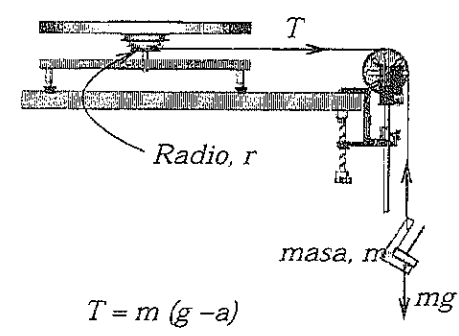
\includegraphics[width=\linewidth]{imagenes/esquema-smart-pulley.png}\par
        {\small (a) Esquema del montaje.}
    \end{minipage}
    \hfill
    \begin{minipage}[b]{0.31\textwidth}
        \centering
        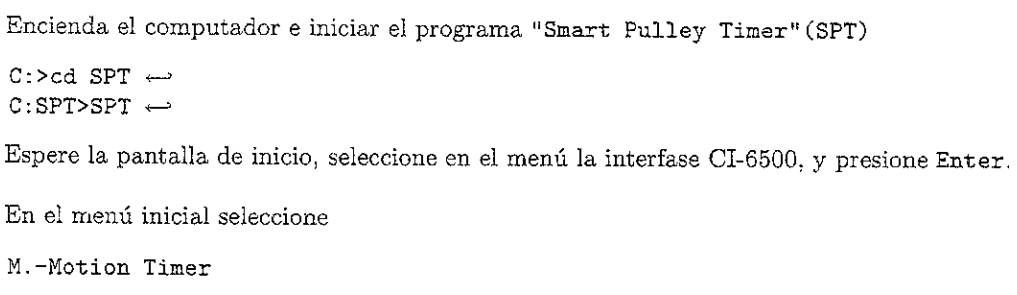
\includegraphics[width=\linewidth]{imagenes/inst.png}\par
        {\small (b) Configuración inicial del programa.}
    \end{minipage}
    \hfill
    \begin{minipage}[b]{0.31\textwidth}
        \centering
        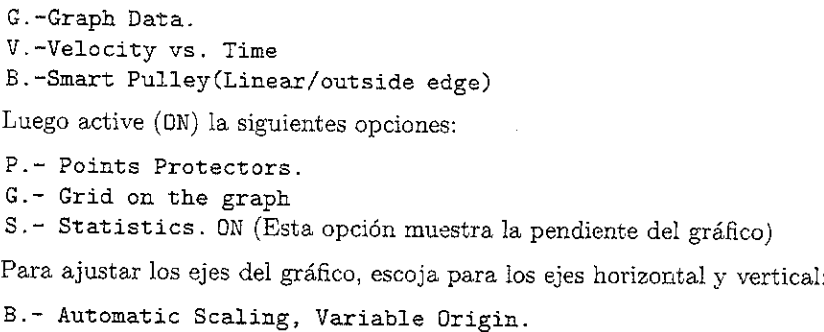
\includegraphics[width=\linewidth]{imagenes/inst2.png}\par
        {\small (c) Herramienta de análisis de datos.}
    \end{minipage}
    \caption{Montaje y adquisición de datos para la medición de aceleraciones tangenciales mediante \textit{Smart Pulley}.}
    \label{fig:montaje-general}
\end{figure*}

\subsection{Procedimiento}

\begin{enumerate}
    \item Se midieron los radios efectivos de enrollamiento $r_1$, $r_2$ y $r_3$.
    \item Se conectó la cuerda al gancho portamasas y se enrolló sobre el radio seleccionado, procurando mantener una altura inicial fija.
    \item Se registró la velocidad tangencial en función del tiempo mediante la \textit{Smart Pulley}.
    \item Para cada masa, se ajustó la curva velocidad-tiempo y se tomó la pendiente como aceleración tangencial $a_t$.
    \item Se repitió el procedimiento tres veces para cada masa y para cada radio.
    \item Se calculó la aceleración angular mediante $\alpha=a_t/r$ y el torque aplicado mediante $\tau=rm(g-r\alpha)$.
\end{enumerate}

\begin{figure}[H]
    \centering
    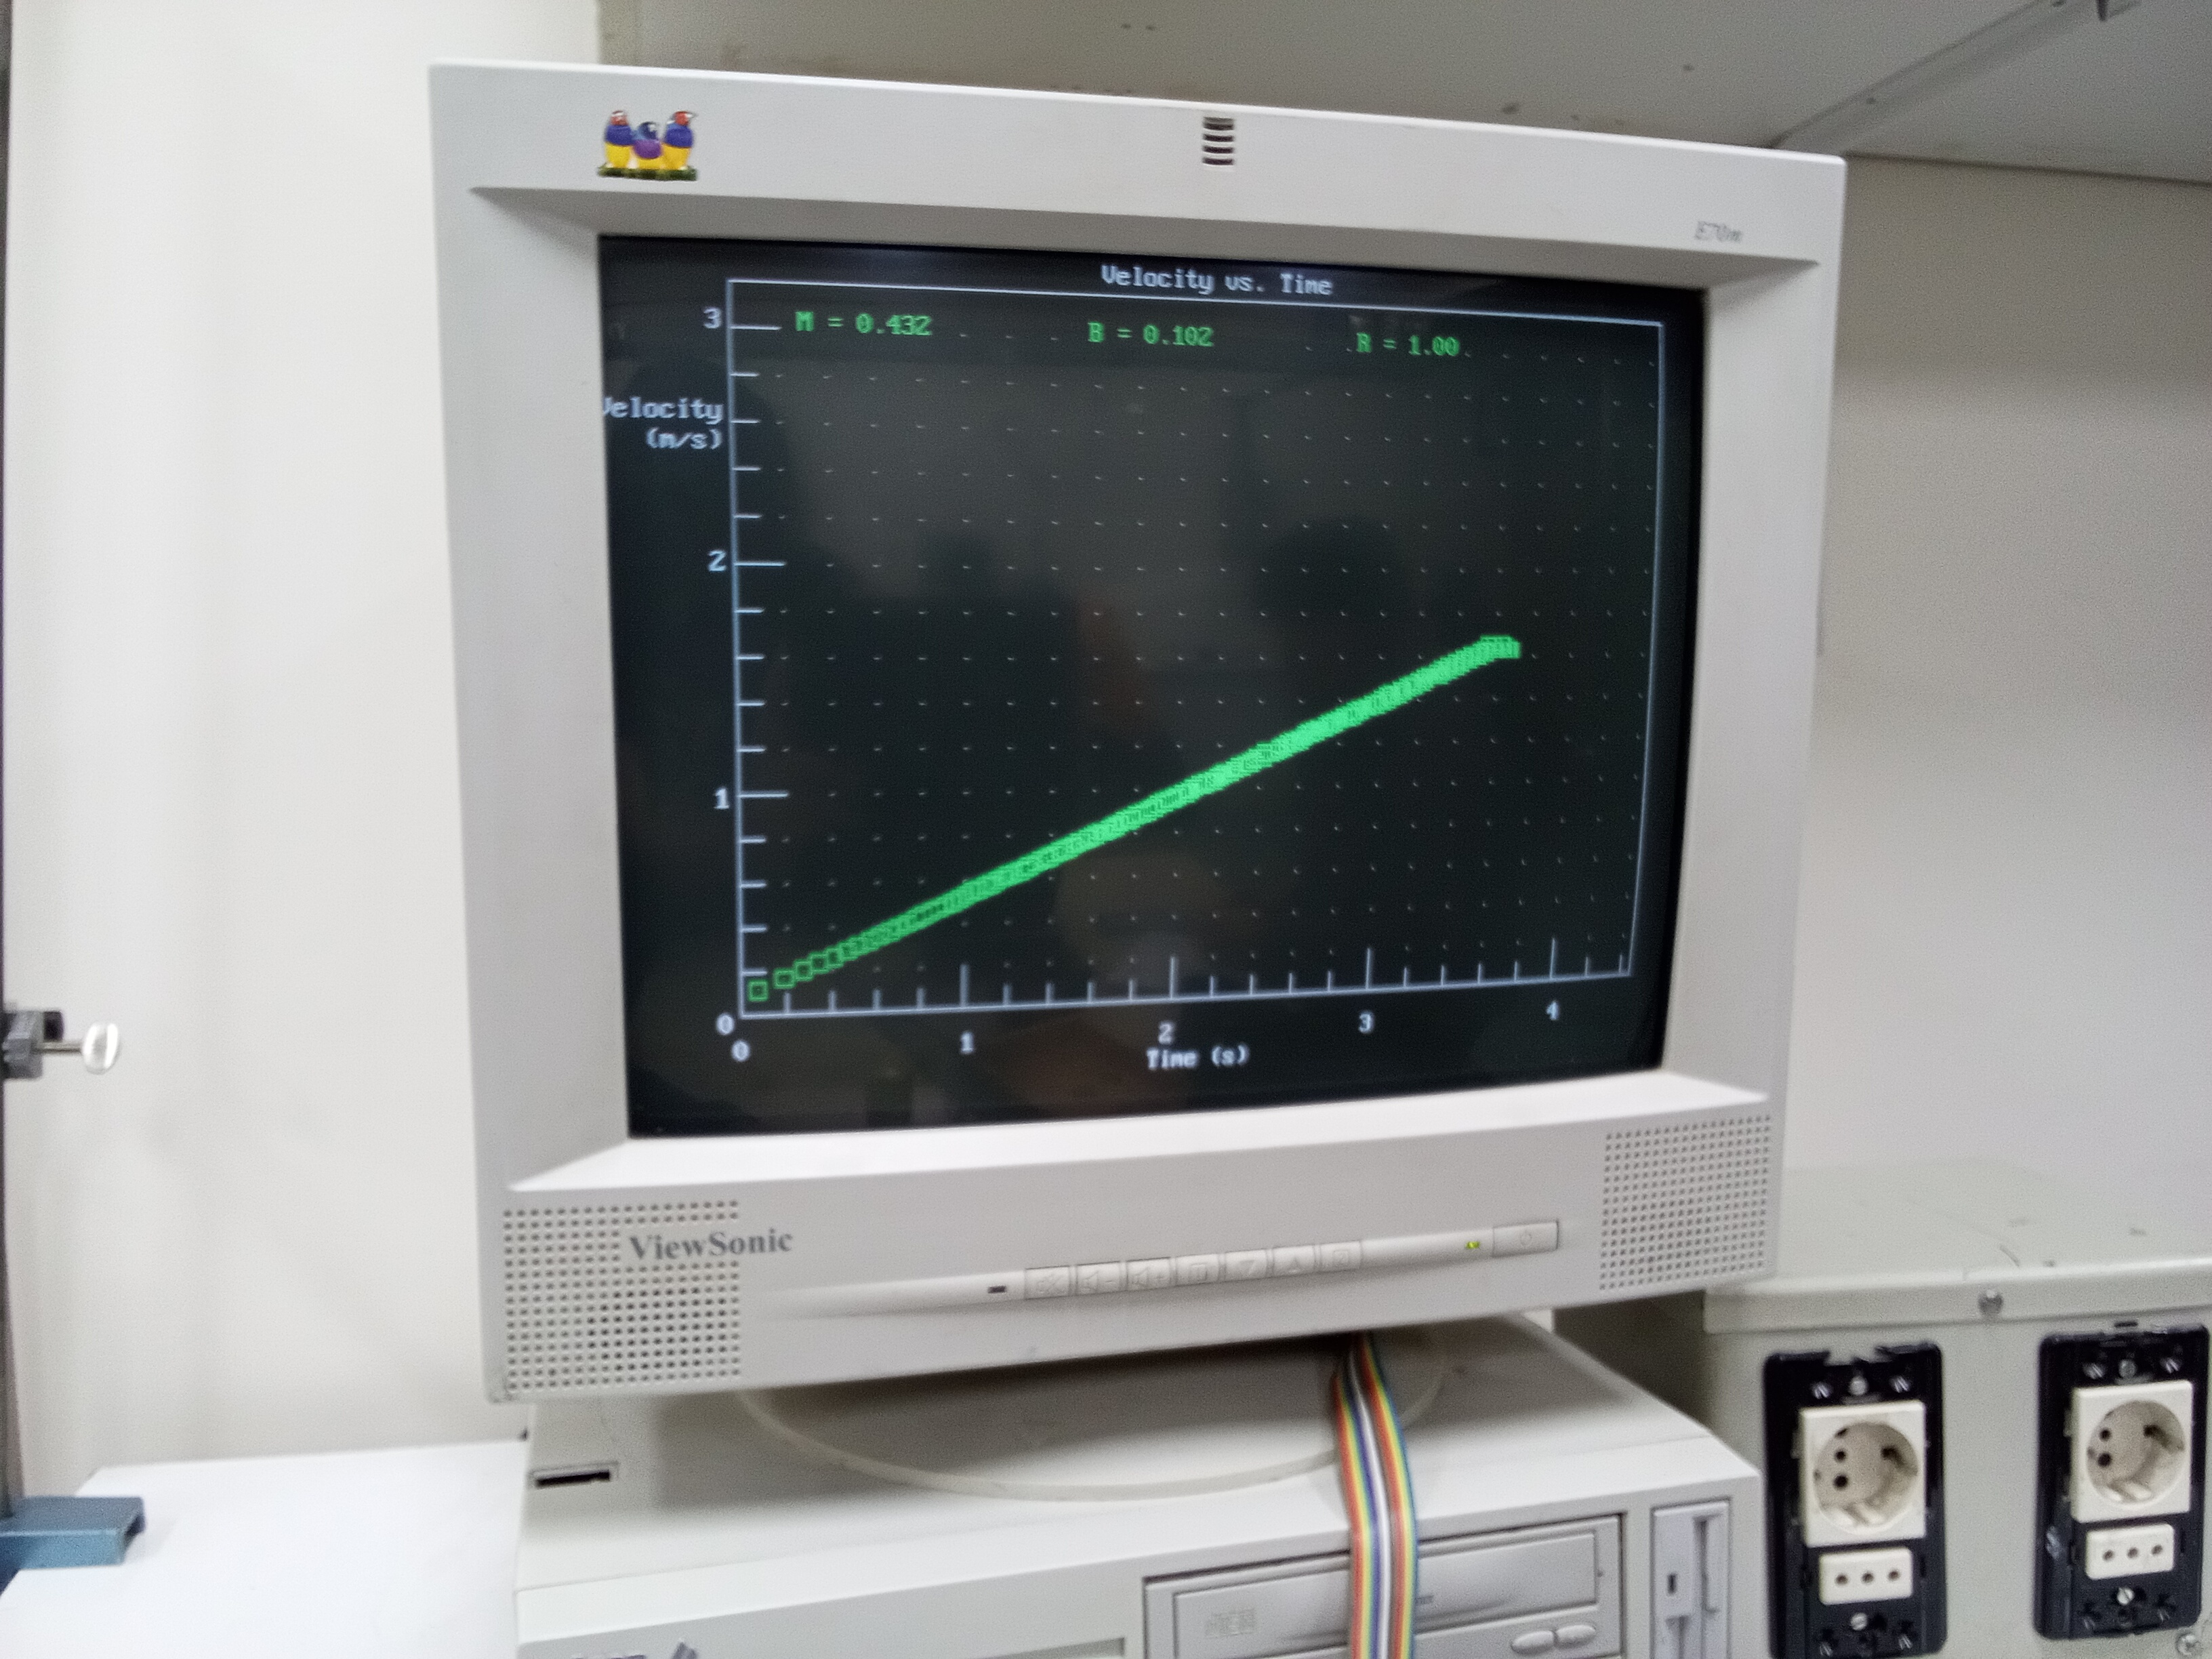
\includegraphics[width=\linewidth]{imagenes/graficoPC-98.jpg}
    \caption{Ejemplo de registro velocidad-tiempo en el sistema de adquisición. La pendiente del ajuste lineal entrega la aceleración tangencial $a_t$.}
    \label{fig:grafico-pc}
\end{figure}

\section{Reporte de datos.}

En el Cuadro \ref{tab:datos-procesados} se presentan los datos procesados usados en el ajuste lineal. Las aceleraciones tangenciales corresponden al promedio de las mediciones repetidas para cada masa y radio. A partir de ellas se calculó $\alpha=a_t/r$ y $\tau=rm(g-r\alpha)$.

\begin{table*}[t]
\centering
\caption{Datos procesados para la determinación experimental del momento de inercia.}
\label{tab:datos-procesados}
\resizebox{\textwidth}{!}{%
\begin{tabular}{cccccc}
\toprule
Radio & Masa $m$ (kg) & Radio $r$ (m) & $a_t$ (m/s$^2$) & $\alpha$ (rad/s$^2$) & $\tau$ (N m) \\
\midrule
$r_1$ & 0.01025 & 0.027 & 0.031 & 1.15 & 0.003 \\
$r_1$ & 0.05000 & 0.027 & 0.194 & 7.17 & 0.013 \\
$r_1$ & 0.06000 & 0.027 & 0.235 & 8.72 & 0.015 \\
$r_1$ & 0.10000 & 0.027 & 0.396 & 14.65 & 0.025 \\
$r_1$ & 0.11000 & 0.027 & 0.434 & 16.09 & 0.027 \\
\midrule
$r_2$ & 0.12000 & 0.022 & 0.403 & 18.30 & 0.025 \\
$r_2$ & 0.13000 & 0.022 & 0.439 & 19.94 & 0.027 \\
$r_2$ & 0.14000 & 0.022 & 0.476 & 21.62 & 0.029 \\
$r_2$ & 0.15000 & 0.022 & 0.494 & 22.45 & 0.030 \\
$r_2$ & 0.16000 & 0.022 & 0.535 & 24.32 & 0.032 \\
\midrule
$r_3$ & 0.12000 & 0.018 & 0.303 & 16.81 & 0.021 \\
$r_3$ & 0.13000 & 0.018 & 0.331 & 18.39 & 0.022 \\
$r_3$ & 0.14000 & 0.018 & 0.354 & 19.67 & 0.024 \\
$r_3$ & 0.15000 & 0.018 & 0.377 & 20.98 & 0.025 \\
$r_3$ & 0.16000 & 0.018 & 0.413 & 22.96 & 0.027 \\
\bottomrule
\end{tabular}%
}
\end{table*}


\section{Análisis de datos.}

\subsection{Ajuste lineal \texorpdfstring{$\tau$ vs. $\alpha$}{tau vs. alpha}}

Para cada radio se graficó el torque aplicado en función de la aceleración angular. El modelo ajustado fue
\begin{equation*}
    \tau(\alpha)=I\alpha+b,
\end{equation*}
donde la pendiente $I$ se interpreta como el momento de inercia experimental y el intercepto $b$ permite detectar posibles contribuciones de torque residual.

\begin{figure*}[t]
    \centering
    \begin{minipage}[b]{0.32\textwidth}
        \centering
        
\includegraphics[width=\linewidth]{imagenes/figure_1.png}\par
        {\small (a) $r_1=\SI{0.027}{m}$.}
    \end{minipage}
    \hfill
    \begin{minipage}[b]{0.32\textwidth}
        \centering
        
\includegraphics[width=\linewidth]{imagenes/figure_2.png}\par
        {\small (b) $r_2=\SI{0.022}{m}$.}
    \end{minipage}
    \hfill
    \begin{minipage}[b]{0.32\textwidth}
        \centering
        
\includegraphics[width=\linewidth]{imagenes/figure_3.png}\par
        {\small (c) $r_3=\SI{0.018}{m}$.}
    \end{minipage}
    \caption{Relación experimental entre torque aplicado y aceleración angular para los tres radios efectivos del sistema.}
    \label{fig:tau-alpha}
\end{figure*}

Los ajustes obtenidos fueron
\begin{align*}
    r_1:&\qquad \tau = 0.001618\,\alpha + 0.001187,\qquad R^2=0.9995,\\
    r_2:&\qquad \tau = 0.001168\,\alpha + 0.003695,\qquad R^2=0.9991,\\
    r_3:&\qquad \tau = 0.001004\,\alpha + 0.003953,\qquad R^2=0.9872.
\end{align*}
La linealidad es clara para los tres radios, por lo que el comportamiento observado es consistente con la forma rotacional de la segunda ley de Newton. El caso $r_3$ presenta una dispersión relativa mayor, lo que puede asociarse a que, para radios más pequeños, pequeñas incertidumbres en $r$ producen variaciones más notorias en $\alpha=a_t/r$ y en $\tau=rm(g-r\alpha)$.

\subsection{Estimación del momento de inercia}

Como la pendiente del ajuste $\tau$ vs. $\alpha$ representa el momento de inercia efectivo, se obtuvo
\begin{align*}
    I_1 &= \SI{1.618e-3}{kg.m^2},\\
    I_2 &= \SI{1.168e-3}{kg.m^2},\\
    I_3 &= \SI{1.004e-3}{kg.m^2}.
\end{align*}
El valor promedio resulta
\begin{align*}
    I_{\mathrm{prom}}
    &=\frac{I_1+I_2+I_3}{3}\\
    &=\frac{0.001618+0.001168+0.001004}{3}\\
    &\approx \SI{1.263e-3}{kg.m^2}.
\end{align*}
Si se compara con el valor de referencia utilizado en el laboratorio,
\begin{equation*}
    I_{\mathrm{ref}}\approx \SI{7.01e-3}{kg.m^2},
\end{equation*}
el error relativo aproximado es
\begin{equation*}
    \varepsilon_I
    =\frac{|I_{\mathrm{prom}}-I_{\mathrm{ref}}|}{I_{\mathrm{ref}}}\times 100\%
    \approx 82\%.
\end{equation*}
La magnitud de esta diferencia sugiere que la principal limitación del experimento no fue la linealidad del ajuste, sino la presencia de errores sistemáticos en la determinación del torque efectivo o de la aceleración angular.

\section{Discusión.}

Los altos valores de $R^2$ muestran que los datos se organizan casi linealmente en el plano $\tau$ vs. $\alpha$. Esto es físicamente importante: aunque el valor absoluto de $I$ difiera del valor de referencia, la tendencia lineal indica que el montaje sí reproduce la estructura esperada de la dinámica rotacional.

La discrepancia en el momento de inercia puede explicarse por varios factores. Primero, el radio que entra en el cálculo no es sólo una longitud geométrica, sino un radio efectivo de enrollamiento de la cuerda. Si la cuerda no se enrolla perfectamente o se superpone sobre sí misma, el radio efectivo cambia durante la caída. Segundo, la fricción en el eje y en la polea introduce un torque adicional que no fue medido de forma independiente. Tercero, el sensor registra una aceleración tangencial asociada al movimiento de la cuerda, de modo que deslizamientos, holguras o errores de calibración se propagan directamente a $\alpha$.

Los interceptos positivos de los ajustes también son relevantes. En un modelo ideal sin fricción ni offset se esperaría $b\simeq0$. Sin embargo, los valores obtenidos indican una contribución residual, compatible con pérdidas mecánicas o con un desplazamiento sistemático en la medición del torque. Por ello, una mejora natural sería medir el torque de fricción por separado y restarlo antes del ajuste, como se recomienda en tratamientos experimentales de incertidumbres y correcciones sistemáticas \cite{taylor1997}.

\section{Conclusiones.}

Se verificó experimentalmente una relación aproximadamente lineal entre el torque aplicado y la aceleración angular para los tres radios considerados. A partir de las pendientes de los ajustes se estimaron momentos de inercia del orden de $10^{-3}\,\si{kg.m^2}$, con un promedio
\begin{equation*}
    I_{\mathrm{prom}}\approx \SI{1.263e-3}{kg.m^2}.
\end{equation*}
La linealidad observada respalda la relación $\tau=I\alpha$ dentro del rango experimental. No obstante, la comparación con el valor de referencia del laboratorio muestra un error relativo grande, cercano al $82\%$, lo que apunta a fuentes sistemáticas de error más que a dispersión aleatoria de los datos.

Para mejorar el experimento se recomienda medir con mayor precisión el radio efectivo de enrollamiento, verificar la calibración de la \textit{Smart Pulley}, estimar el torque de fricción mediante corridas auxiliares y repetir las mediciones controlando que la cuerda no deslice ni cambie de radio durante la caída. Estas correcciones permitirían conservar la buena linealidad observada y, al mismo tiempo, mejorar la estimación absoluta del momento de inercia.

\section*{Apéndice: cálculo por mínimos cuadrados.}
\addcontentsline{toc}{section}{Apéndice: cálculo por mínimos cuadrados}

Para ajustar el modelo lineal
\begin{equation*}
    y=ax+b
\end{equation*}
a un conjunto de datos $(x_i,y_i)$, se minimiza
\begin{equation*}
    S(a,b)=\sum_{i=1}^{n}\left[y_i-(ax_i+b)\right]^2.
\end{equation*}
En este informe se identifica $x_i=\alpha_i$ y $y_i=\tau_i$. La pendiente $a$ entrega el momento de inercia experimental $I$, mientras que el intercepto $b$ representa un posible offset de torque. La calidad del ajuste se evaluó mediante el coeficiente de determinación
\begin{equation*}
    R^2=1-\frac{\sum_i (y_i-y_i^{\mathrm{fit}})^2}{\sum_i (y_i-\overline{y})^2}.
\end{equation*}

\begingroup\scriptsize
\printbibliography[title={Referencias}]
\endgroup

\end{document}
